\documentclass[11pt]{article}
\usepackage{charter}
\usepackage{graphicx}
\usepackage{hyperref}
\usepackage{mdframed}
\usepackage[margin=1in]{geometry}
\usepackage{amsmath}

\hypersetup{
	colorlinks=true,
	linkcolor=blue,
	filecolor=magenta,
	urlcolor=cyan,
}

\begin{document}

%===================================================
% Title and Author Info
%===================================================
\begin{center}
{\Large\textsc{Stable Keplerian Orbits}} \\
\vspace{10pt}
{\large \textbf{Mentor:} Alex Urban} \\
{\small LIGO Laboratory, California Institute of Technology \\
Pasadena, CA 91125, USA \\
\href{mailto:aurban@ligo.caltech.edu}{\texttt{aurban@ligo.caltech.edu}}}
\end{center}

%%%%%%%%%%%%%%%%%%%%%%%%%%%%%%%%%%%%%%%%%%%%%%%%%%%

\section*{Purpose}

\hspace{15pt} In this problem, we will work out the total energy of a stable Keplerian orbit and simulate it in Python. The goal is, once again, to use what we understand now to inform what we're going to do next: with a growing intuition for the astrophysics of compact binaries, we will now implement an awesome Keplerian orbit simulation.... \textit{of science!}

\section*{Stable Keplerian Orbits}
\hspace{15pt} Suppose that a neutron star binary (each with mass $M = 1.4\,\, M_{\odot}$) is in a stable, Keplerian orbit (\textit{i.e.} with no loss of energy). Figure \ref{fig:binary_diagram} illustrates this system.

\begin{figure}[!h]
\begin{mdframed}
\centering
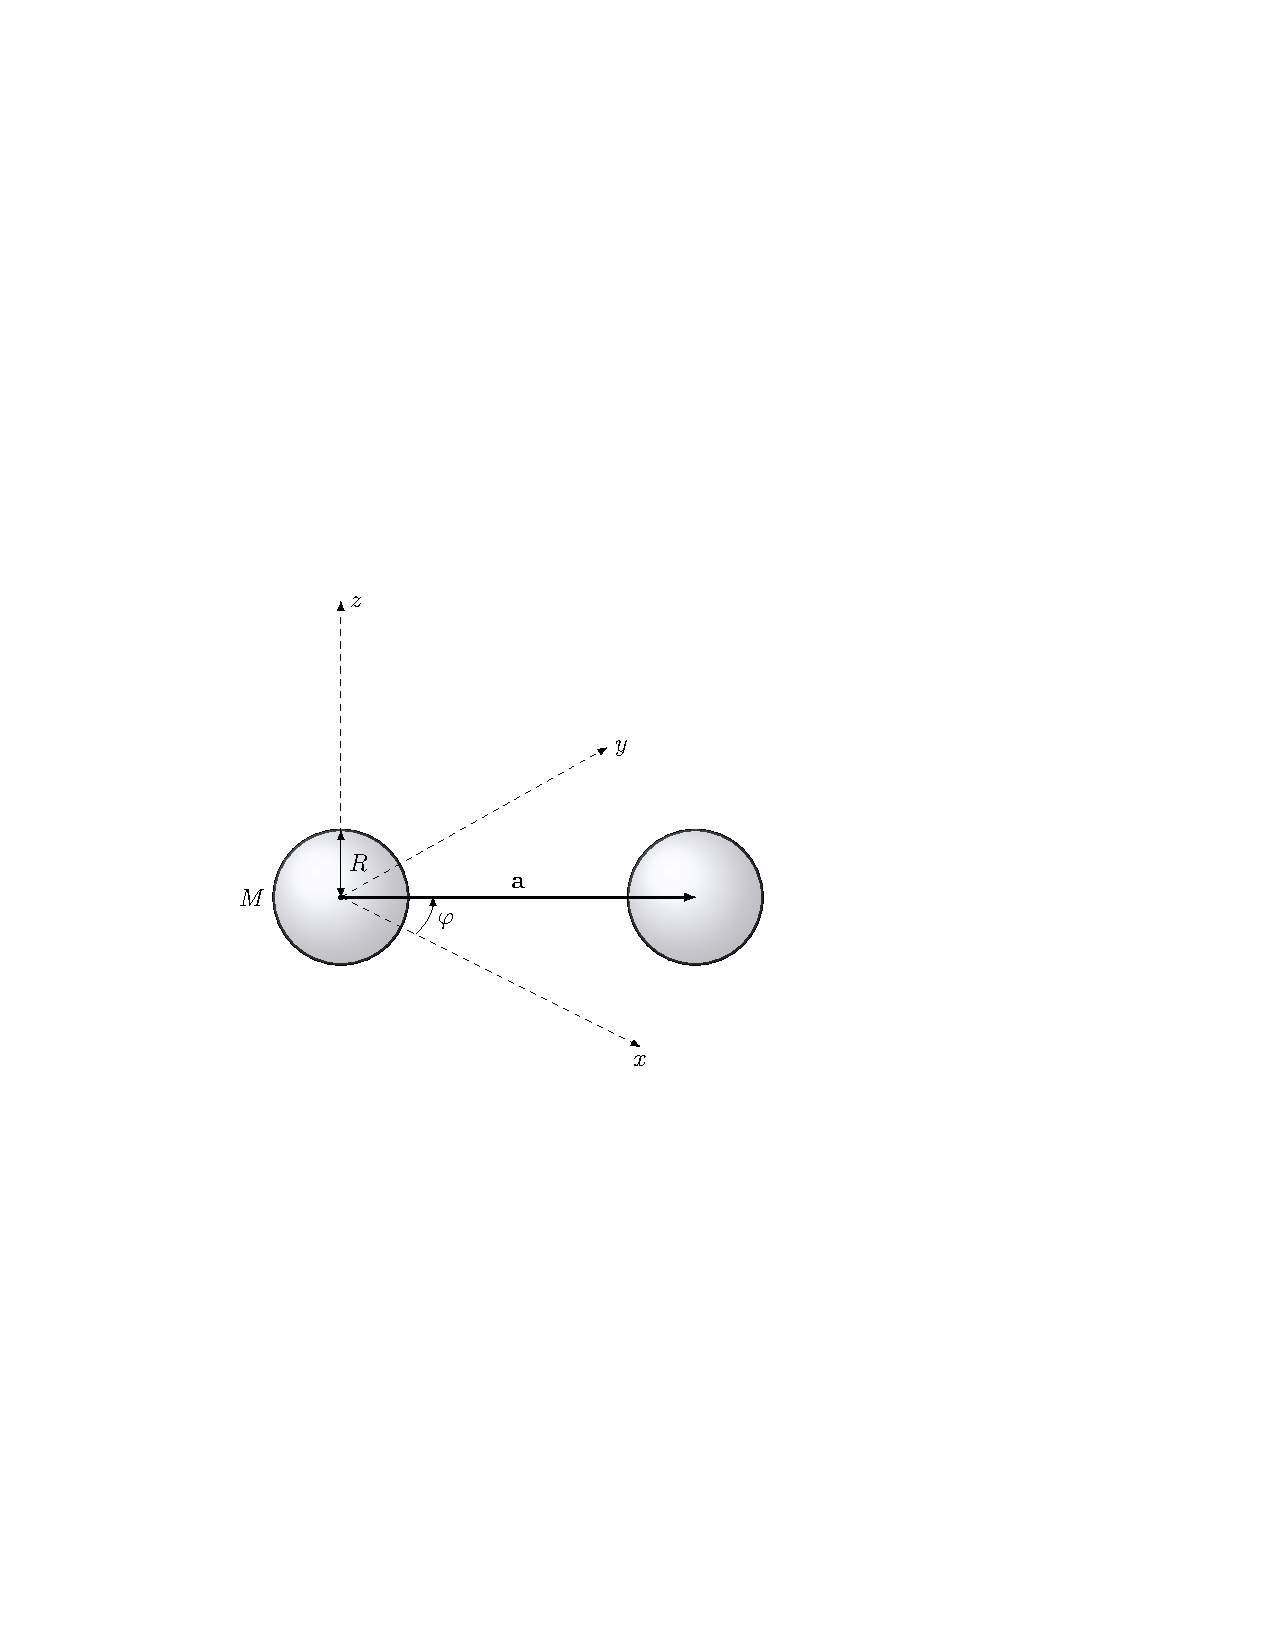
\includegraphics{stable_orbit/binary_diagram.pdf}
\caption{\label{fig:binary_diagram}Diagram of the neutron star binary, showing its orbital separation ($a$) and the radius ($R$) and masses ($M$) of the individual neutron stars. The various mutual gravitational forces at play are also illustrated.}
\end{mdframed}
\end{figure}

\begin{enumerate}

\item Using Kepler's laws, show that when the orbit is perfectly circular, the azimuthal angle $\varphi$ is a linear function of time. (You can presume the orbit is in a plane, so $\theta = \pi/2 =$ const.)

\item Write the angular velocity $\omega = d\varphi/dt$ in terms of $a$ and the orbital angular momentum, $L$, and plot $L$ and $v=a\omega$ \textit{vs.} the gravitational wave frequency for circular orbits. (Remember that the LIGO instruments are sensitive to binary neutron stars up to about 3000 or 4000 Hz, so that should be the range of your plot.)

\item Show that if $a$ is allowed to vary (still with no energy loss!), then the total energy is
\begin{equation}
E = \frac{M}{4}\left(\frac{da}{dt}\right)^2 + \Phi(a; L)
\end{equation}
where the function
\begin{equation}\label{eq:effective_potential}
\Phi(a; L) = - \frac{GM^2}{a} + \frac{L^2}{Ma^2}
\end{equation}
is called the \textit{effective potential}. (Note that $L$ is conserved during a Keplerian orbit, so the effective potential only depends on $a$.)

\item Find the critical points of $\Phi$ with respect to $a$, and plot the effective potential for $2L^2/GM^3 =$ 0, 20, 40, and 60 km. What physics do these critical points tell us? How can we interpret the term in $\Phi$ that depends on $L^2$?

\item Try writing a Python simulation using \href{https://en.wikipedia.org/wiki/Euler_method}{Euler's method} to integrate the equations for $a$ and $\varphi$ using arbitrary values for $E$, $L$, and the initial velocity. As a sanity check, your simulation should plot the total energy and orbital angular momentum (both should be constant), along with $a$, $\varphi$, and the orbital velocity, all as a function of time. The simulation should also draw complete orbits in polar coordinates, experimenting with different initial conditions.

\item Now, combine these results with last week's. What energies and angular momenta give us stable circular orbits in the region where 30 Hz $\leq f_{\rm GW} \leq$ 3000 Hz? What does the centrifugal force on each neutron star look like in this region? How does this compare with the tidal force?

\end{enumerate}

\section*{Things That Make You Go, ``Hmmm....''}

\begin{enumerate}

\item What elements do you think are still missing from our understanding of neutron star binary mergers?

\item Can you argue on the basis of symmetry that it's valid to restrict Keplerian orbital motion to a plane?

\item Can you think of a physical motivation for why we expect neutron star binaries to be in stable circular orbits?

\item Suppose we add to this system a tiny point particle of mass $m \ll M$. What do you think its motion would look like in different regions?

\end{enumerate}

%%%%%%%%%%%%%%%%%%%%%%%%%%%%%%%%%%%%%%%%%%%%%%%%%%%

\vspace{1000pt}

\subsection*{Solution}

\begin{enumerate}

\item From Kepler's first law, we know that all closed orbits are elliptical in shape. For those orbits that are perfectly circular, this means the orbital separation $a =$ constant. Kepler's second law then tells us that a line connecting the two bodies sweeps out equal areas in equal times; when the orbit is perfectly circular, this must imply that $\omega = d\varphi/dt =$ constant since $\varphi$ is the only coordinate changing over time. It follows that \textbf{during circular orbits},
\begin{equation}
\varphi(t) = \omega t + \varphi_0
\end{equation}
where $\omega = 2\pi f_{\rm orbital}$ and $\varphi_0$ are constants, as desired.

\item As seen in Figure \ref{fig:binary_diagram}, the gravitational force affects a total relative acceleration \[ \frac{d^2\mathbf{a}}{dt^2} = \frac{\mathbf{F}_{\rm 21}}{M} - \frac{\mathbf{F}_{\rm 12}}{M} = \frac{2}{M}\,\mathbf{F}_{\rm g} \] where $\mathbf{F}_{\rm g}$ is the (mutual) gravitational force of one neutron star on the other and $\mathbf{a}$ is the separation vector between them. Since gravitation is a central force, the relative acceleration must be purely radial; that is, there can be no angular component of acceleration on one star relative to the other. Since we already presumed orbital motion is planar (why?) this must mean that the $\varphi$ component of acceleration vanishes, so there can be no net torque: \[ 2a\,\frac{da}{dt}\,\frac{d\varphi}{dt} + a^2\,\frac{d^2\varphi}{dt^2} = \frac{d}{dt} \left( a^2\,\frac{d\varphi}{dt} \right) = 0. \]
The term in parentheses is $a$ times the perpendicular component of velocity, which you might remember as the orbital angular momentum $L$ of one neutron star,
\begin{equation}
\frac{2}{M}\, \mathbf{L} = \mathbf{a} \times \mathbf{v} = a^2\,\frac{d\varphi}{dt} \, \hat{\mathbf{z}},
\end{equation}
where $\mathbf{v}$ is the instantaneous linear velocity of one star relative to the other and $\hat{\mathbf{z}}$ is a unit vector perpendicular to the orbital plane. This statement can be interpreted as saying that \textbf{orbital angular momentum is conserved} during a generic Keplerian orbit.

\hspace{15pt} Recall that during circular orbits, the gravitational wave frequency is twice the orbital frequency ($f_{\rm GW} = 2f_{\rm orbital}$). Since $\omega = 2\pi f_{\rm orbital} = \pi f_{\rm GW}$ by definition, and since we know
\begin{equation}
a = \left[ \frac{2GM}{(\pi f_{\rm GW})^2} \right]^{1/3}
\end{equation}
from last week's work, the orbital velocity of each body is
\begin{equation}
v = a\omega = \pi a f_{\rm GW} = \left( 2\pi GMf_{\rm GW} \right)^{1/3}
\end{equation}
and the orbital angular momentum is
\begin{equation}
L = \frac{M}{2} a^2 \omega = \left( \frac{G^2M^{5}}{2\pi f_{\rm GW}} \right)^{1/3}
\end{equation}
during stable circular orbits. These quantities are plotted in Figure \ref{fig:L}.

\begin{figure}
\centering
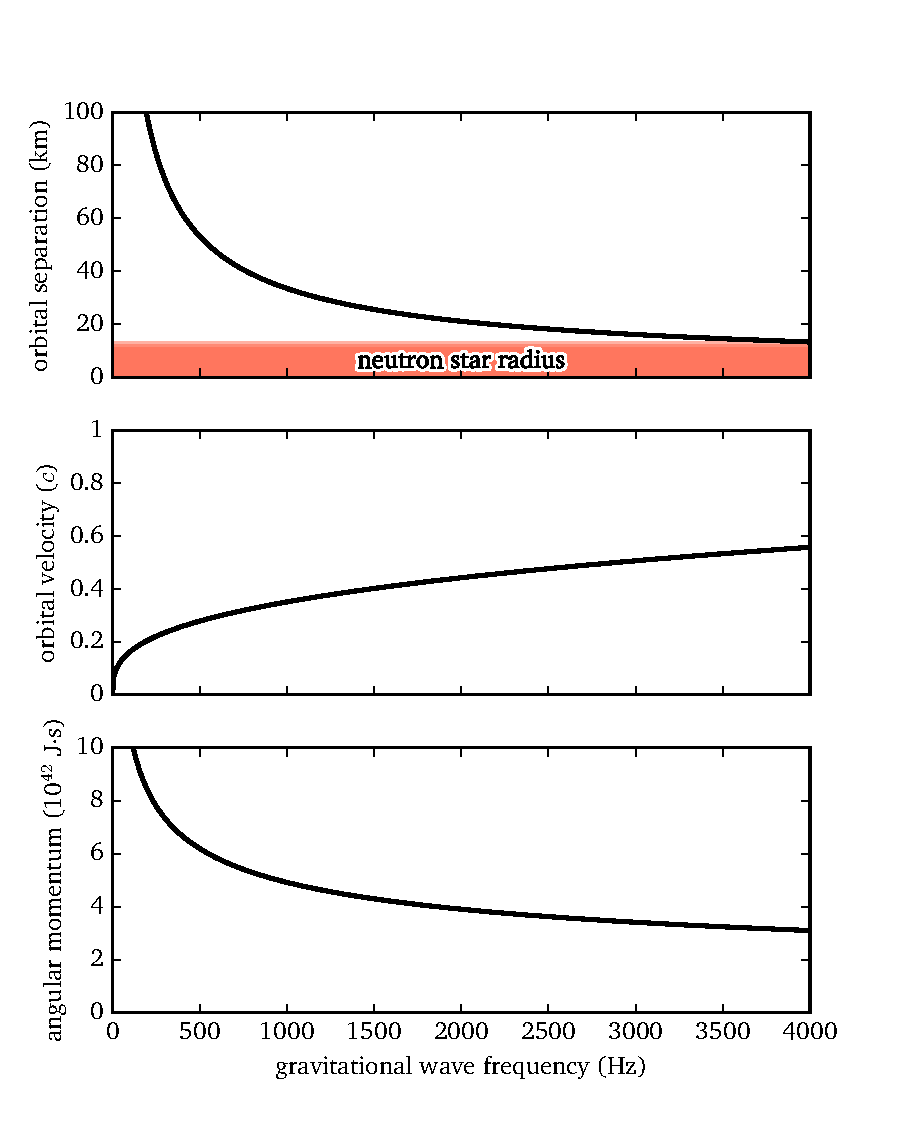
\includegraphics[scale=1]{stable_orbit/kepler_angular_momentum.pdf}
\caption{\label{fig:L} Various features of circular Keplerian orbits expressed as a function of the gravitational wave frequency. Top: orbital separation; \textit{i.e.} the distance between neutron star cores. Middle: orbital velocity, expressed as a fraction of the speed of light, $c$. (Note the incredibly extreme speeds attained by neutron stars in LIGO's sensitive frequency band.) Bottom: orbital angular momentum (solid) and total energy (dashed; see Eq. \ref{eq:energy}), which once again is quite extreme.}
\end{figure}

\item To make the problem simpler we can write down the total energy of one neutron star relative to the other, thinking in terms of the total mass $M_{\rm tot} = 2M$ and the ``reduced'' mass $\mu = M/2$ as in question (2) above. Because of the symmetry of the system we know that the center of mass lives exactly midway between the two neutron stars at all times, meaning a particle at the center of mass has no kinetic energy. Thus, the total energy of an equivalent one-body system is \[ E = \frac{\mu}{2} \left[ \left(\frac{da}{dt}\right)^2 + a^2\omega^2 \right] - \frac{GM^2}{a}. \] But, we also know that the total angular momentum $L = \mu a^2\omega$ is conserved during a given orbit, so we can re-write the total energy in terms of $a$, its derivative, and $L$:
\begin{equation}
E = \frac{M}{4}\left(\frac{da}{dt}\right)^2 - \frac{GM^2}{a} + \frac{L^2}{Ma^2}
\end{equation}
as we set out to show. (The last two terms constitute the effective potential in Eq. \ref{eq:effective_potential}.) Note, because of Newton's third law and the symmetry of the system, the motion of star 2 relative to star 1 will mirror the motion of star 1 relative to star 2.

\begin{figure}[!b]
\centering
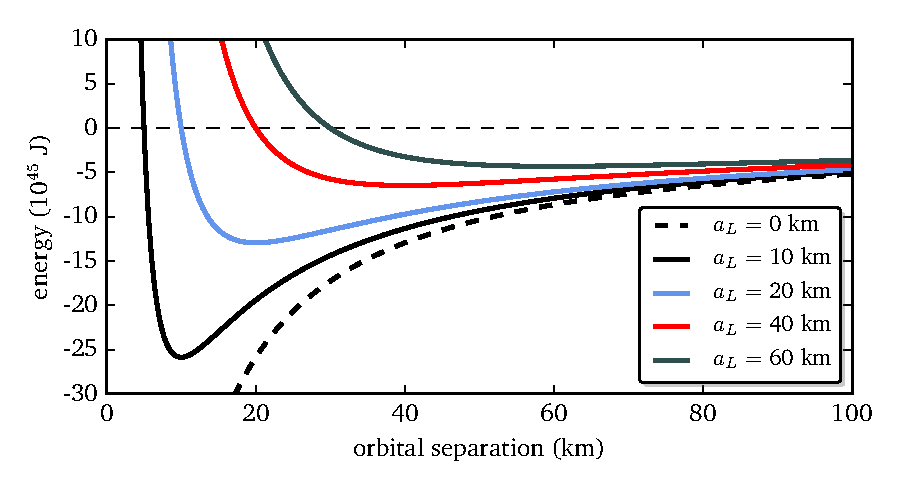
\includegraphics[scale=1]{stable_orbit/kepler_potentials.pdf}
\caption{\label{fig:potentials} Effective potential as a function of orbital separation for various values of the total angular momentum, $L$, expressed in terms of the stable circular orbit radius $a_L = 2L^2/GM^3$. Note the colossal energy scale of $\sim$10$^{46}$ J available to close neutron star binaries.}
\end{figure}

\item See Figure \ref{fig:potentials} for a plot of the effective potential with different total angular momentum values. The critical points of $\Phi$ are local minima where its first derivative goes to zero, $d\Phi/da = 0$, providing stable circular orbits with orbital separation
\begin{equation}\label{eq:aL}
a_L = \frac{2L^2}{GM^3}.
\end{equation}
Physically, this means the total energy is
\begin{equation}\label{eq:energy}
E_L = -\frac{GM^2}{2a_L} = - \left( \frac{GM^{5/2}}{2L} \right)^2
\end{equation} for stable circular orbits (see Figure \ref{fig:L}), implying that close circular orbits require less angular momentum and have more gravitational binding energy than more distant ones.

\hspace{15pt} The last term in the effective potential looks like $L^2/Ma^2$, which can loosely be thought of as summoning a central force
\begin{equation}
\mathbf{F}_{\rm c}(a; L) = -\frac{\partial\Phi}{\partial a} \, \hat{\mathbf{a}} = \frac{2L^2}{Ma^3} \, \hat{\mathbf{a}}
\end{equation}
pushing outward against each neutron star. (Here $\hat{\mathbf{a}} = \mathbf{a}/a$.) This is a \textit{centrifugal force} caused by angular motion that balances the radial pull of gravity and creates an effective 1-dimensional potential barrier at $a < a_L$, so that \emph{all} orbits (both open and closed) have an inner turning point. \textbf{Remember this, because we will revisit it when we add in the effects of general relativity.} The magnitude of orbital centrifugal force as a function of $f_{\rm GW}$ is visualized in Figure \ref{fig:forces}.

\hspace{15pt} Always remember that the centrifugal term in $\Phi$ is really a form of kinetic energy, and that the centrifugal ``force'' is an artifact of non-inertial motion.

\begin{figure}[!h]
\centering
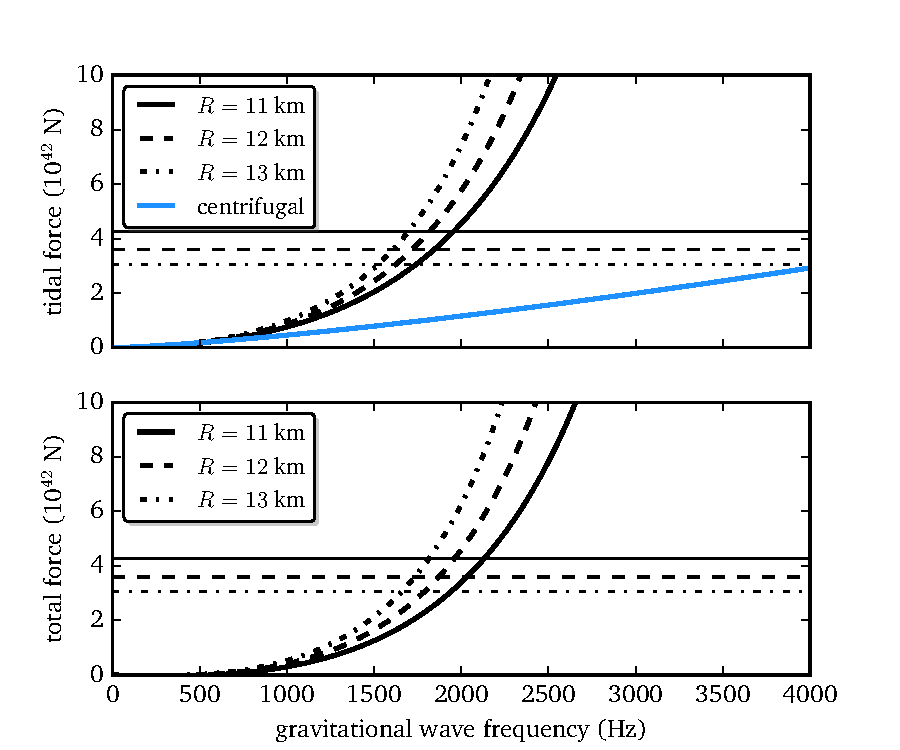
\includegraphics[scale=1]{stable_orbit/kepler_centrifugal_force.pdf}
\caption{\label{fig:forces} The various forces (in Newtons) on one neutron star due to the pull of the other, compared at different neutron star radii. Top: tidal forces due to a rapidly changing gravitational field gradient, and the centrifugal force due to orbital motion, shown separately. Bottom: the sum of tidal (attractive) and centrifugal (repulsive) forces. Horizontal lines show the neutron star's total self-binding force.}
\end{figure}

\item Recall that Euler's method is an algorithm for integrating simple 1-dimensional differential equations by doing the most naive thing possible: if \[ \frac{df}{dt} = g(f; t) \] is a first-order differential equation relating some function $f$ to itself and the independent variable $t$, then Euler's method approximates its solution by gridding up the domain into $N$ uniform steps $t_i = 0, h, \dots, (N-1)h$ of (small) length $h$, and then summing over them: \[ f(t_i) = f(t_{i-1}) + h\,g(f(t_{i-1}), t_{i-1}). \]
The idea is that the approximation converges to the true integral as $h \rightarrow 0$, by definition of a derivative. Euler's method is not perfect, and we will explore its shortcomings and limitations together as well as other integration schemes (or ``integrators''), but for right now, it will serve our purposes well.

\hspace{15pt} In order to use Euler's method, we first need to specify some initial conditions. For the problem at hand, we actually have a system of coupled nonlinear equations to solve simultaneously:
\begin{align*}
\frac{da}{dt} &= \pm \sqrt{ \frac{4}{M} \left[ E - \Phi(a; L) \right] } \\
\frac{d\varphi}{dt} &= \frac{2L}{Ma^2}.
\end{align*}
A unique orbit for one of the neutron stars is completely specified by starting values $a(t_0)$ and $\varphi(t_0)$, total energy $E$, and orbital angular momentum $L$. By symmetry, the other star \emph{has to} mirror the orbit of this one.

\hspace{2pt} Solving the orbit equations analytically in closed form is simply not possible. Fortunately, with Euler's method we can get pretty good approximate solutions, and this is much easier than it sounds. But there are a couple of subtleties (there's always a catch!):
\begin{enumerate}
\item We need to make sure we have adequate \textit{time resolution} (the step size, $h$) in order to capture highly dynamic astrophysics.

\item The total energy is quadratic in $da/dt$, so we need to be scrupulously mindful of sign flips.
\end{enumerate}
We can get around both of these issues by wisely applying the physical intuition we've been developing in the past couple of weeks.

\hspace{15pt}I have an example simulation \href{https://github.com/alurban/mentoring/blob/master/tidal_distortion/scripts/kepler_orbits.py}{in GitHub}, which I wrote in Python. I used a fixed angular momentum of $L=$ 4$\times$10$^{42}$ J$\cdot$s, a range of total energies between 0 and $E_L$ (Eq. \ref{eq:energy}), and initial values $a(t_0) = a_L$ (Eq. \ref{eq:aL}) and $\varphi(t_0) = 0$. For each orbit, I used a step size equal to 0.005\% of $P_{\rm circular}$ (the period we expect for stable circular orbits), and chose the initial velocity to be negative (\textit{i.e.} falling toward the other neutron star). I then followed each orbit for 15$P_{\rm circular}$. The results are shown in Figures \ref{fig:simulated_parameters}, \ref{fig:sanity_checks}, \ref{fig:trace}, and \ref{fig:trace_unbound}. We will pour through each of these results together in great detail, but in the meantime, you should look at them closely on your own.

\end{enumerate}

%%%%%%%%%%%%%%%%%%%%%%%%%%%%%%%%%%%%%%%%%%%%%%%%%%%

\begin{mdframed}
\vspace{-15pt}

\section*{Things That Make You Go, ``Hmmm....''}

\begin{enumerate}

\item What elements do you think are still missing from our understanding of neutron star binary mergers?

\item Can you argue on the basis of symmetry that it's valid to restrict Keplerian orbital motion to a plane?

\item Can you think of a physical motivation for why we expect neutron star binaries to be in stable circular orbits?

\item Suppose we add to this system a tiny point particle of mass $m \ll M$. What do you think its motion would look like in different regions?

\end{enumerate}

\end{mdframed}

%%%%%%%%%%%%%%%%%%%%%%%%%%%%%%%%%%%%%%%%%%%%%%%%%%%

\vspace{1000pt}

\begin{figure}[!h]
\centering
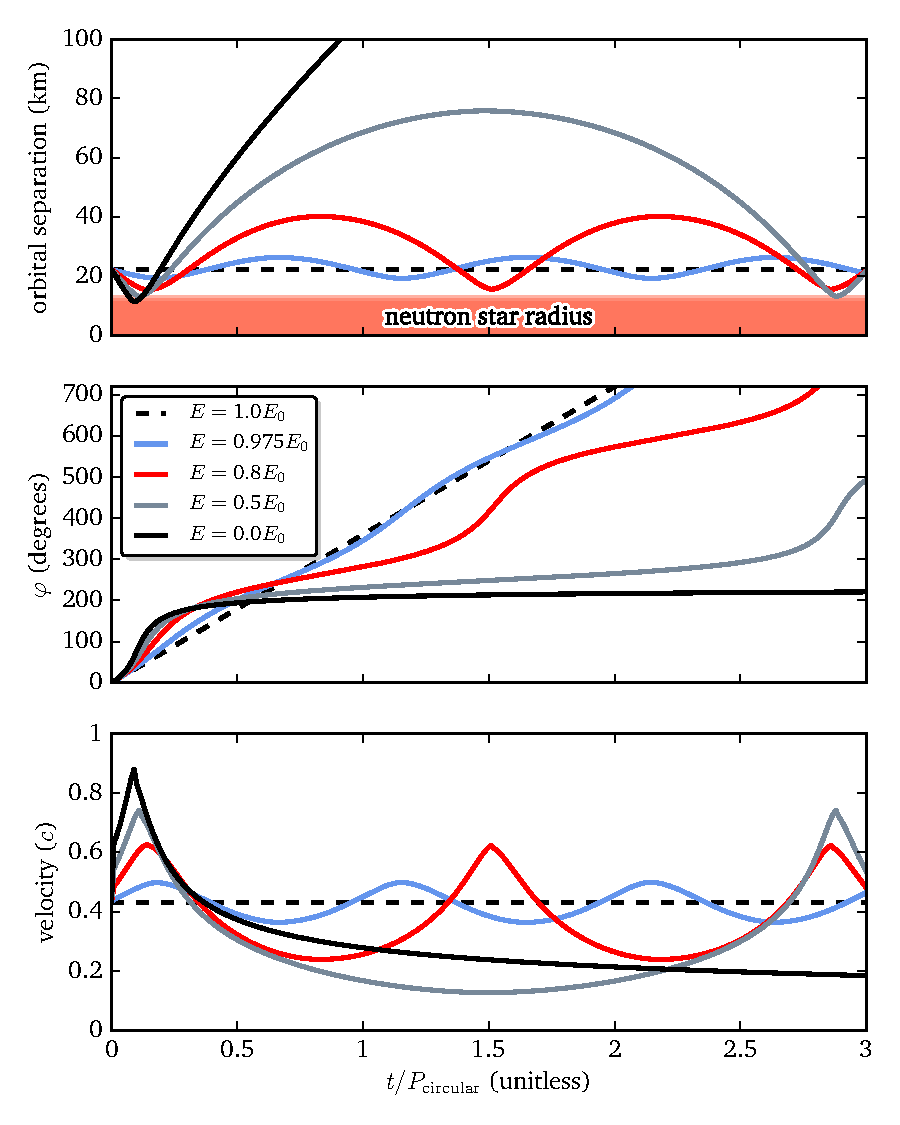
\includegraphics[scale=1]{stable_orbit/orbit_parameters.pdf}
\caption{\label{fig:simulated_parameters} Features of each simulated orbit as approximated by Euler's method. Top: orbital separation, with the radius of the other neutron star shown for reference. Note the orbit with $E=$ 0.99$E_L$ looks like a sinusoid in $a$ with about the same period as $P_{\rm circular}$ -- this is no accident. (Can you think of why?) Middle: the polar angle $\varphi(t)$. Bottom: instantaneous orbital velocity expressed as a fraction of the speed of light.}
\end{figure}

\begin{figure}[!h]
\centering
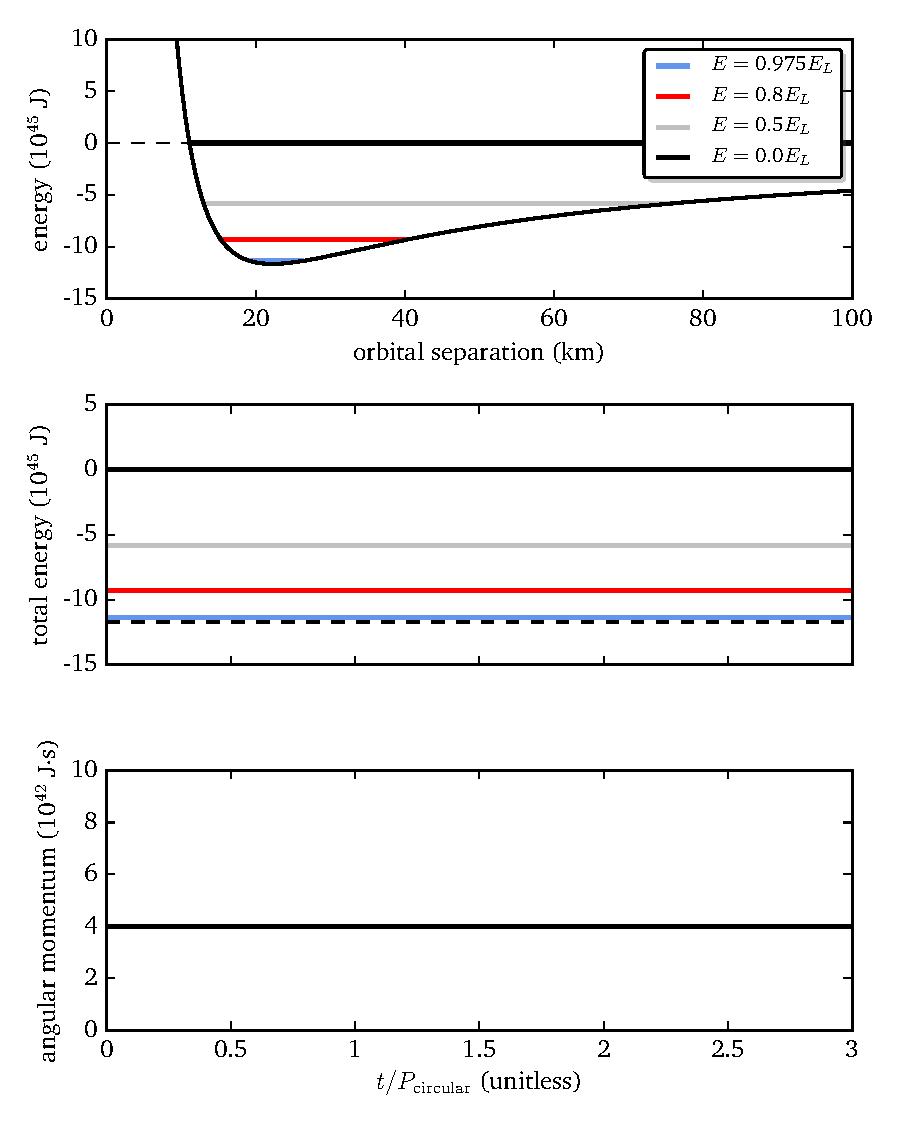
\includegraphics[scale=1]{stable_orbit/sanity_checks.pdf}
\caption{\label{fig:sanity_checks} Sanity checks on the stability and accuracy of this simulation with Euler's method. Top: an effective potential diagram with the simulated energy levels indicated. Note that one circular orbit, three elliptical orbits, and one marginally bound parabolic orbit were done successfully. Middle and bottom: energy and angular momentum as calculated from the approximate solutions for $a$ and $\varphi$. Note that both $E$ and $L$ are successfully conserved in all cases.}
\end{figure}

\begin{figure}[!h]
\centering
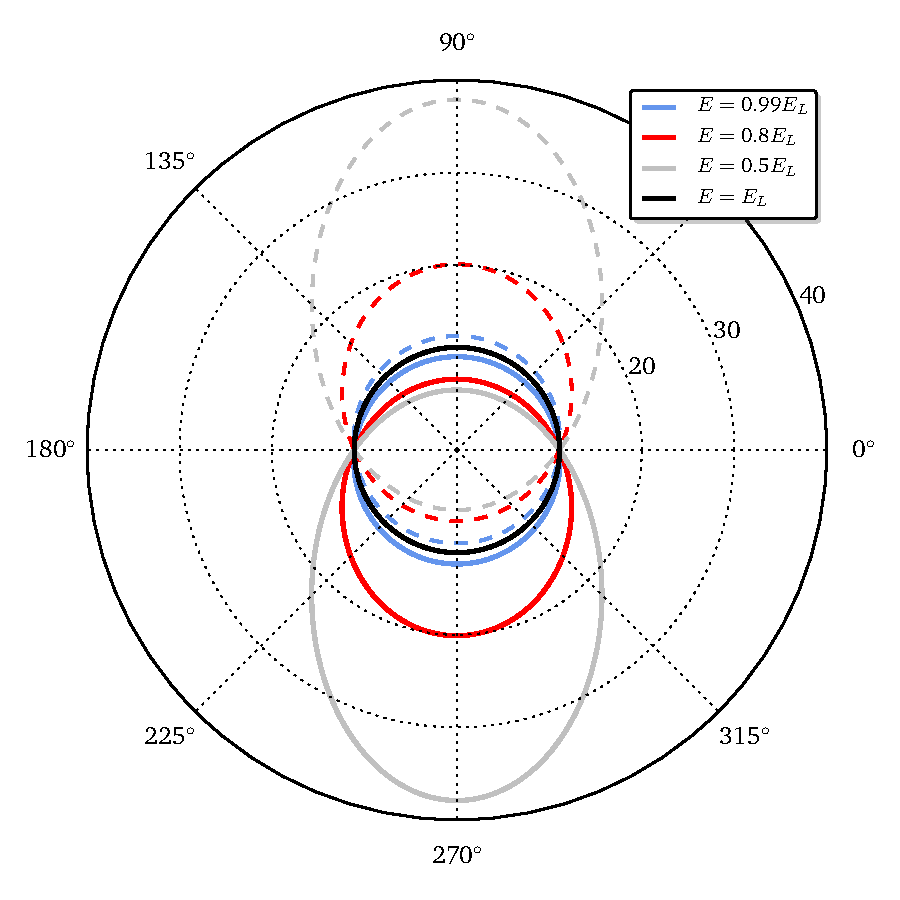
\includegraphics[scale=1]{stable_orbit/orbit_diagram.pdf}
\caption{\label{fig:trace} Traces of the four closed orbits I simulated on a polar diagram. The circular orbit is at a radius $a_L \approx 20$ km. (Note that when you use too high a step size during elliptical orbits, the perihelion advances clockwise around the orbital plane -- this is unphysical behavior that is actually impossible in Keplerian orbits.)}
\end{figure}

\begin{figure}[!h]
\centering
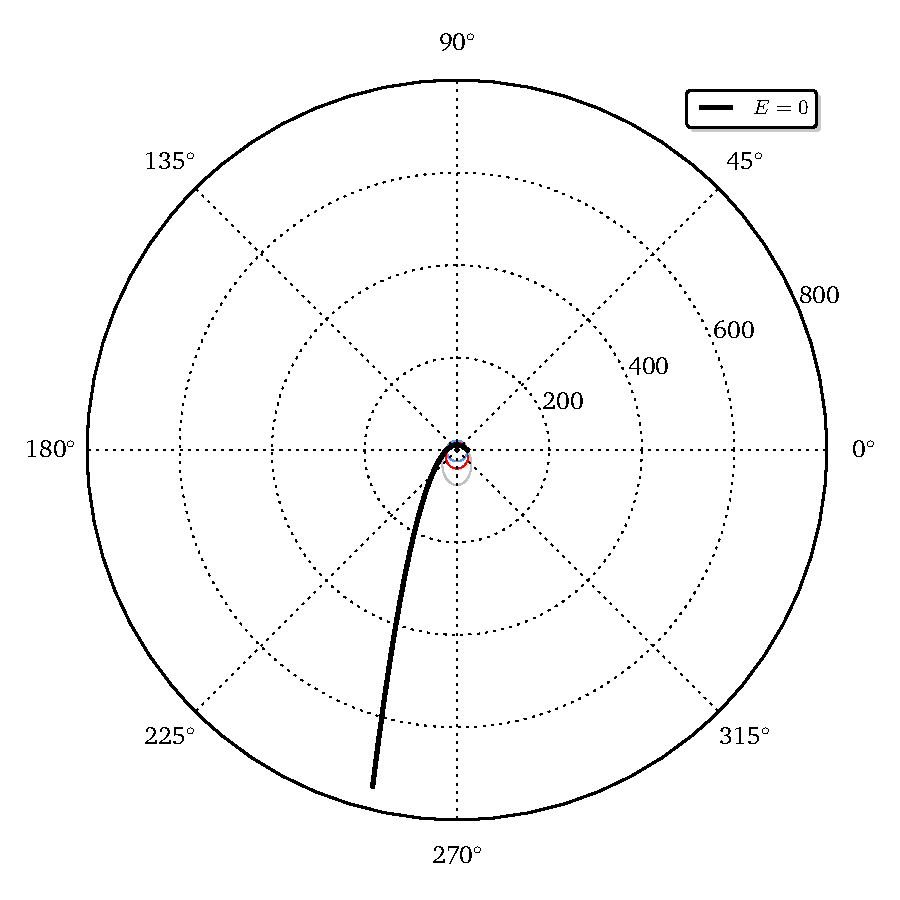
\includegraphics[scale=1]{stable_orbit/orbit_diagram_unbound.pdf}
\caption{\label{fig:trace_unbound} Trace of the marginally bound parabolic orbit with $E=0$. Note the way this orbit starts at $a_L$ and rapidly gets shot way out of range; in this case the neutron star would continue escaping to infinity. Traces of the other elliptical orbits are shown for reference. (The parabolic orbit was followed out to around $a\approx 800$ km.)}
\end{figure}

\end{document}
